\documentclass[a4paper,oneside,14pt]{article}

\usepackage{cmap} % Улучшенный поиск русских слов в полученном pdf-файле
\usepackage[T2A]{fontenc} % Поддержка русских букв
\usepackage[utf8]{inputenc} % Кодировка utf8
\usepackage[english,russian]{babel} % Языки: русский, английский
\usepackage{CJKutf8}

\usepackage[14pt]{extsizes}

\usepackage[table]{xcolor}

\usepackage{graphicx}
\usepackage{multirow}

\usepackage{caption}
\captionsetup{labelsep=endash}
\captionsetup[figure]{name={Рисунок}}

\usepackage{amsmath}
\usepackage{amsfonts}

\usepackage{geometry}
\geometry{left=25mm}
\geometry{right=25mm}
\geometry{top=25mm}
\geometry{bottom=25mm}

\usepackage{alphabeta}
\usepackage{enumitem}
\AddEnumerateCounter{\asbuk}{\@asbuk}{м}

\usepackage{tabularx}

% Переопределение стандартных \section, \subsection, \subsubsection по ГОСТу;

% \usepackage{titlesec}
\usepackage{titlesec}[explicit]
\titleformat{name=\section,numberless}[block]{\normalfont\large\bfseries\centering}{}{0pt}{}
\titleformat{\section}[block]{\normalfont\large\bfseries}{\thesection}{1em}{}
\titlespacing\section{\parindent}{*4}{*4}

\titleformat{\subsection}[hang]
{\bfseries\large}{\thesubsection}{1em}{}
\titlespacing\subsection{\parindent}{*2}{*2}

\titleformat{\subsubsection}[hang]
{\bfseries\large}{\thesubsubsection}{1em}{}
\titlespacing\subsubsection{\parindent}{*2}{*2}

\usepackage{url}

% Переопределение их отступов до и после для 1.5 интервала во всем документе
\usepackage{setspace}
\onehalfspacing % Полуторный интервал
\frenchspacing
\setlength\parindent{1.25cm}

\usepackage{indentfirst} % Красная строка

% Настройки оглавления
% \usepackage{xcolor}
% \usepackage[table]{xcolor}
\usepackage{multirow}
\usepackage{longtable}

% Гиперссылки
\usepackage[pdftex]{hyperref}
% \usepackage[xetex]{hyperref}
% \usepackage{hyperref}
\hypersetup{hidelinks}

% \numberwithin{equation}{section}

% Дополнительное окружения для подписей
\usepackage{array}
\newenvironment{signstabular}[1][1]{
	\renewcommand*{\arraystretch}{#1}
	\tabular
}{
	\endtabular
}

\usepackage{enumitem} 
\setenumerate[0]{label=\arabic*)} % Изменение вида нумерации списков
\renewcommand{\labelitemi}{---}

% Листинги 
\usepackage{courier}

\usepackage{float}
\usepackage{listings}
\floatstyle{plaintop}
\newfloat{code}{H}{myc}

\usepackage{chngcntr} % Listings counter within section set main.tex after begin document

% Для листинга кода:
\lstset{
	basicstyle=\small\ttfamily,			% размер и начертание шрифта для подсветки кода
	language=SQL,   					% выбор языка для подсветки	
	numbers=left,						% где поставить нумерацию строк (слева\справа)
	numbersep=5pt,
	% stepnumber=1,						% размер шага между двумя номерами строк
	xleftmargin=17pt,
	% showstringspaces=false,
	numbersep=5pt,						% как далеко отстоят номера строк от подсвечиваемого кода
	frame=single,						% рисовать рамку вокруг кода
	tabsize=4,							% размер табуляции по умолчанию равен 4 пробелам
	captionpos=b,						% позиция заголовка вверху [t] или внизу [b]
	breaklines=true,					
	breakatwhitespace=true,				% переносить строки только если есть пробел
	escapeinside={\#*}{*)},				% если нужно добавить комментарии в коде
	inputencoding=utf8x,
	backgroundcolor=\color{white},
	numberstyle=,%\tiny,					    % размер шрифта для номеров строк
	% keywordstyle=\color{blue},
	keywordstyle=\color{black},
	% stringstyle=\color{red!90!black}, % color of text in ""
	stringstyle=\color{black}, % color of text in ""
	% commentstyle=\color{green!50!black},
	commentstyle=\color{black},
    morekeywords={TO,WITH,SUPERUSER,PRIVILEGES,TABLES,SCHEMA,USER,PASSWORD,public,REFERENCES,UUID,IF}
}

\lstdefinelanguage{Golang}%
  {morekeywords=[1]{package,import,func,type,struct,return,defer,panic,%
     recover,select,var,const,iota,},%
   morekeywords=[2]{string,uint,uint8,uint16,uint32,uint64,int,int8,int16,%
     int32,int64,bool,float32,float64,complex64,complex128,byte,rune,uintptr,%
     error,interface},%
   morekeywords=[3]{map,slice,make,new,nil,len,cap,copy,close,true,false,%
     delete,append,real,imag,complex,chan,},%
   morekeywords=[4]{for,break,continue,range,go,goto,switch,case,fallthrough,if,%
     else,default,},%
   morekeywords=[5]{Println,Printf,Error,Print,},%
   sensitive=true,%
   morecomment=[l]{//},%
   morecomment=[s]{/*}{*/},%
   morestring=[b]',%
   morestring=[b]",%
   morestring=[s]{`}{`},%
}

\lstset{
	literate=
	{а}{{\selectfont\char224}}1
	{б}{{\selectfont\char225}}1
	{в}{{\selectfont\char226}}1
	{г}{{\selectfont\char227}}1
	{д}{{\selectfont\char228}}1
	{е}{{\selectfont\char229}}1
	{ё}{{\"e}}1
	{ж}{{\selectfont\char230}}1
	{з}{{\selectfont\char231}}1
	{и}{{\selectfont\char232}}1
	{й}{{\selectfont\char233}}1
	{к}{{\selectfont\char234}}1
	{л}{{\selectfont\char235}}1
	{м}{{\selectfont\char236}}1
	{н}{{\selectfont\char237}}1
	{о}{{\selectfont\char238}}1
	{п}{{\selectfont\char239}}1
	{р}{{\selectfont\char240}}1
	{с}{{\selectfont\char241}}1
	{т}{{\selectfont\char242}}1
	{у}{{\selectfont\char243}}1
	{ф}{{\selectfont\char244}}1
	{х}{{\selectfont\char245}}1
	{ц}{{\selectfont\char246}}1
	{ч}{{\selectfont\char247}}1
	{ш}{{\selectfont\char248}}1
	{щ}{{\selectfont\char249}}1
	{ъ}{{\selectfont\char250}}1
	{ы}{{\selectfont\char251}}1
	{ь}{{\selectfont\char252}}1
	{э}{{\selectfont\char253}}1
	{ю}{{\selectfont\char254}}1
	{я}{{\selectfont\char255}}1
	{А}{{\selectfont\char192}}1
	{Б}{{\selectfont\char193}}1
	{В}{{\selectfont\char194}}1
	{Г}{{\selectfont\char195}}1
	{Д}{{\selectfont\char196}}1
	{Е}{{\selectfont\char197}}1
	{Ё}{{\"E}}1
	{Ж}{{\selectfont\char198}}1
	{З}{{\selectfont\char199}}1
	{И}{{\selectfont\char200}}1
	{Й}{{\selectfont\char201}}1
	{К}{{\selectfont\char202}}1
	{Л}{{\selectfont\char203}}1
	{М}{{\selectfont\char204}}1
	{Н}{{\selectfont\char205}}1
	{О}{{\selectfont\char206}}1
	{П}{{\selectfont\char207}}1
	{Р}{{\selectfont\char208}}1
	{С}{{\selectfont\char209}}1
	{Т}{{\selectfont\char210}}1
	{У}{{\selectfont\char211}}1
	{Ф}{{\selectfont\char212}}1
	{Х}{{\selectfont\char213}}1
	{Ц}{{\selectfont\char214}}1
	{Ч}{{\selectfont\char215}}1
	{Ш}{{\selectfont\char216}}1
	{Щ}{{\selectfont\char217}}1
	{Ъ}{{\selectfont\char218}}1
	{Ы}{{\selectfont\char219}}1
	{Ь}{{\selectfont\char220}}1
	{Э}{{\selectfont\char221}}1
	{Ю}{{\selectfont\char222}}1
	{Я}{{\selectfont\char223}}1
}

% Работа с изображениями и таблицами; переопределение названий по ГОСТу
\usepackage{caption}
\captionsetup[figure]{name={Рисунок},labelsep=endash}
% \captionsetup[table]{singlelinecheck=false, labelsep=endash}
\captionsetup[table]{justification=raggedright, singlelinecheck=false, labelsep=endash}

\usepackage[justification=centering]{caption} % Настройка подписей float объектов	

\usepackage{csvsimple}

\usepackage{ulem} % Нормальное нижнее подчеркивание
\usepackage{hhline} % Двойная горизонтальная линия в таблицах
\usepackage[figure,table]{totalcount} % Подсчет изображений, таблиц
\usepackage{rotating} % Поворот изображения вместе с названием
\usepackage{lastpage} % Для подсчета числа страниц

\makeatletter
% \renewcommand\@biblabel[1]{#1.} % [1] -> 1. in bibliography
\makeatother

\usepackage{float} % Place figures anywhere you want; ignore floating

\usepackage{ragged2e} % Перенос слов на следующую строку
\usepackage{pdfpages}

\usepackage{threeparttable}

\usepackage{blindtext}

% CW-specific

\usepackage{xparse} % \NewDocumentCommand for creating custom commands

% \usepackage{tabularx}
\usepackage{adjustbox} % Hyperlinks
% \usepackage[table]{xcolor}

\renewcommand{\underset}[2]{\ensuremath{\mathop{\mbox{#2}}\limits_{\mbox{\scriptsize #1}}}} % Use \underset in normal environment, not only in math

% Write stuff under underlined text
\NewDocumentCommand{\ulinetext}{O{3cm} O{c} m m} % O - optional; m - mandatory
{\underset{#3}{\uline{\makebox[#1][#2]{#4}}}}

% Font configuration
% \usepackage{fontspec}
% \setmainfont{Liberation Serif} % Liberation Serif} % ~ Times New Roman
% \setsansfont{Roboto} % Liberation Sans} % ~ Arial
% \setsansfont{Liberation Sans} % ~ Arial
% \setmonofont{Liberation Mono} % ~ Courier New

\usepackage{totcount}

% Подсчет количества рисунков и таблиц
\regtotcounter{figure}
\regtotcounter{table}


\begin{document}

\noindent
\textbf{Проектирование базы данных для разметчиков параллельного корпуса технических текстов}

\noindent
\textbf{Рунов Константин Алексеевич} \hfill runovka@student.bmstu.ru

\noindent
\textit{МГТУ им. Н. Э. Баумана, Москва, 105005, Россия}

% Аннотация
\noindent
% \textit{В статье рассмотрены актуальные проблемы разметчиков параллельных корпусов технических текстов и предложен вариант проектирования базы данных для решения некоторых из них}
\textit{В статье рассмотрены актуальные проблемы разметчиков параллельных корпусов технических текстов, рассмотрена функциональность информационной системы для решения некоторых из них, представлена диаграмма сущностей базы данных для описанной информационной системы, и приведен сценарий использования системы}

\noindent
Ключевые слова:
% \noindent
\textit{
    корпусная лингвистика,
    параллельные корпуса текстов,
    терминологическая разметка,
    база данных
}

% \vfill

\noindent
\textbf{Design of database for parallel corpora of technical texts annotators}

\noindent
\textbf{Runov Konstantin Alexeevich} \hfill runovka@student.bmstu.ru

\noindent
\textit{BMSTU, 105005, Russia}

% Annotation
\noindent
\textit{The article considers actual problems of parallel corpora of technical texts annotators, considers the functionality of the information system for solving some of them, presents the diagram of database entities for the described information system, and gives a scenario of the system usage}
% \textit{The paper covers actual problems of parallel corpora of technical texts annota-tors and proposes an option of database design for the solution of some of them}

\noindent
Keywords:
% \noindent
corpus linguistics,
parallel corpora,
terminological markup,
database

% \newpage

% Основной текст статьи
\textbf{Введение}

На сегодняшний день корпусная лингвистика является неотъемлемой частью лингвистики, науки о языке~\cite{cl2020}.
Корпуса текстов находят применение в различных областях --- в машинном переводе, в разработке словарей, в лингвистических исследованиях.
Для того, чтобы из корпуса текстов можно было извлекать пользу, тексты в нем должны быть размечены.
Существуют различные алгоритмы, позволяющие автоматически производить разметку текстов, но для проверки ее корректности все равно, как правило, требуется вмешательство человека.

На данный момент не существует открытых параллельных корпусов технических текстов, а также инструментов для автоматической разметки русскоязычных текстов~\cite{butenko2020-2, butenko2022}.
Это делает актуальным разработку информационной системы для участников разметки параллельного корпуса технических текстов.
% , а также информационных систем, позволяющих одновременно
% \begin{itemize}
%     \item производить разметку текста в параллельном корпусе,
%     \item производить поиск по параллельному корпусу,
%     \item организовать удобное взаимодействие участников разметки,
% \end{itemize}
% что делает актуальным разработку таковой.

Целью данной статьи является создание диаграммы сущностей базы данных для информационной системы, предназначенной для участников разметки параллельного корпуса технических текстов.

Для достижения поставленной цели, будут
\begin{itemize}
    \item рассмотрены актуальные проблемы, с которыми сталкиваются участники разметки параллельных корпусов технических текстов, 
    \item описана функциональность информационной системы, позволяющей организовать удобную работу множества участников разметки параллельного корпуса технических текстов,
    % \item предложена диаграмма сущностей базы данных для описанной информационной системы.
    \item выделены сущности базы данных для описанной информационной системы.
\end{itemize}

% \textbf{Актуальные проблемы разметки параллельных корпусов технических текстов участниками разметки}
\textbf{Проблемы разметки параллельных корпусов технических текстов}

% Кроме отсутствия открытых параллельных корпусов технических текстов и информационных систем для организации удобной работы множества участников разметки, существуют также проблемы, относящиеся к автоматизации проведения терминологической разметки.
% Так, при попытке определения границ терминов, возникает целый ряд проблем.

% Актуальными проблемами разметки параллельных корпусов технических текстов являются проблемы, возникающие при попытке автоматического определения границ терминов.
Актуальные проблемы разметки параллельных корпусов технических текстов связаны с автоматическим определением границ терминов.
Среди них выделяют~\cite{butenko2022}:
\begin{itemize}
    \item неправильное определение границ терминов-словосочетаний, состоящих из двух и более слов и составных терминов; 
    \item распознавание составных терминов и терминов-словосочетаний, состоящих из двух и более слов;
    \item определение лексической единицы как термина в зависимости от контекста и тематики текста, в котором данная лексическая единица употребляется; 
    \item объемные списки терминов-кандидатов, которые необходимо проверять вручную.
\end{itemize}

% Точность определения границ термина при автоматической разметке является одной из основных лингвистических задач, а отсутствие на сегодняшний день информационных систем для автоматической разметки русскоязычных текстов делает актуальным разработку таковой.
Точность определения границ термина при автоматической разметке является одной из основных лингвистических задач, но на сегодняшний день отсутствуют информационные системы для автоматической разметки русскоязычных текстов~\cite{butenko2022}.

\textbf{Существующие параллельные корпуса текстов и информационные системы для разметки текстов}

Существует множество параллельных корпусов (My-Memory, Opus, Linguee, Glosbe, Reverso, TAUS Data Cloud и др.)~\cite{butenko2020-1}, сервисов для автоматического выравнивания текстов (Hunalign, Euclid, Abbyy Aligner, Trados, Winalign, Wordfast tools, Giza++ и др.)~\cite{cl2020},
% служб, позволяющих создавать собственные корпусы и производить в них поиск (SketchEngine~\cite{ske}, NoSketchEngine~\cite{noske});
инструментов для автоматического извлечения терминов (TerMine, TermExtraction, Termino-logy Extraction)~\cite{butenko2022}.
% и прочих инструментов для работы с корпусами текстов (OpenCorpora~\cite{opencorpora}).
Однако не существует открытых параллельных корпусов технических текстов, а также инструментов для проведения автоматической разметки русскоязычных текстов.

% Но на данный момент не существует открытых параллельных корпусов технических текстов~\cite{butenko2020-2}.
% Также нет открытых информационных систем, позволяющих одновременно производить разметку текста в параллельном корпусе, производить поиск по параллельному корпусу и организовать удобную работу множества разметчиков.

% \textbf{Функциональность информационной системы для участников разметки параллельных корпусов технических текстов}
\textbf{Функциональность информационной системы для участников разметки параллельного корпуса технических текстов}

Для организации удобной работы множества участников разметки параллельного корпуса технических текстов, информационная система должна обладать рядом функций, которые можно разделить на три категории --- функции пользователя, функции модератора и функции администратора.

Администратор системы имеет полный доступ к данным: может добавлять, удалять тексты, добавлять, удалять, изменять разметки, назначать новых модераторов.

Модератор может создавать, изменять и удалять задания на разметку, а также производить проверку разметки, после чего либо утверждать, либо отклонять ее.

Пользователь может выполнять задания на разметку, просматривать выполненные разметки, производить поиск по корпусу.

Каждый пользователь имеет свой рейтинг доверия, который растет с увеличением количества его утвержденных разметок.

% \textbf{Сущности базы данных для разметки параллельных корпусов технических текстов}
\textbf{Сущности базы данных для описанной информационной системы и сценарий использования}

На рисунке \ref{fig:chen} предложен вариант диаграммы сущностей базы данных для описанной информационной системы.

\begin{figure}[H]
	\centering
	% 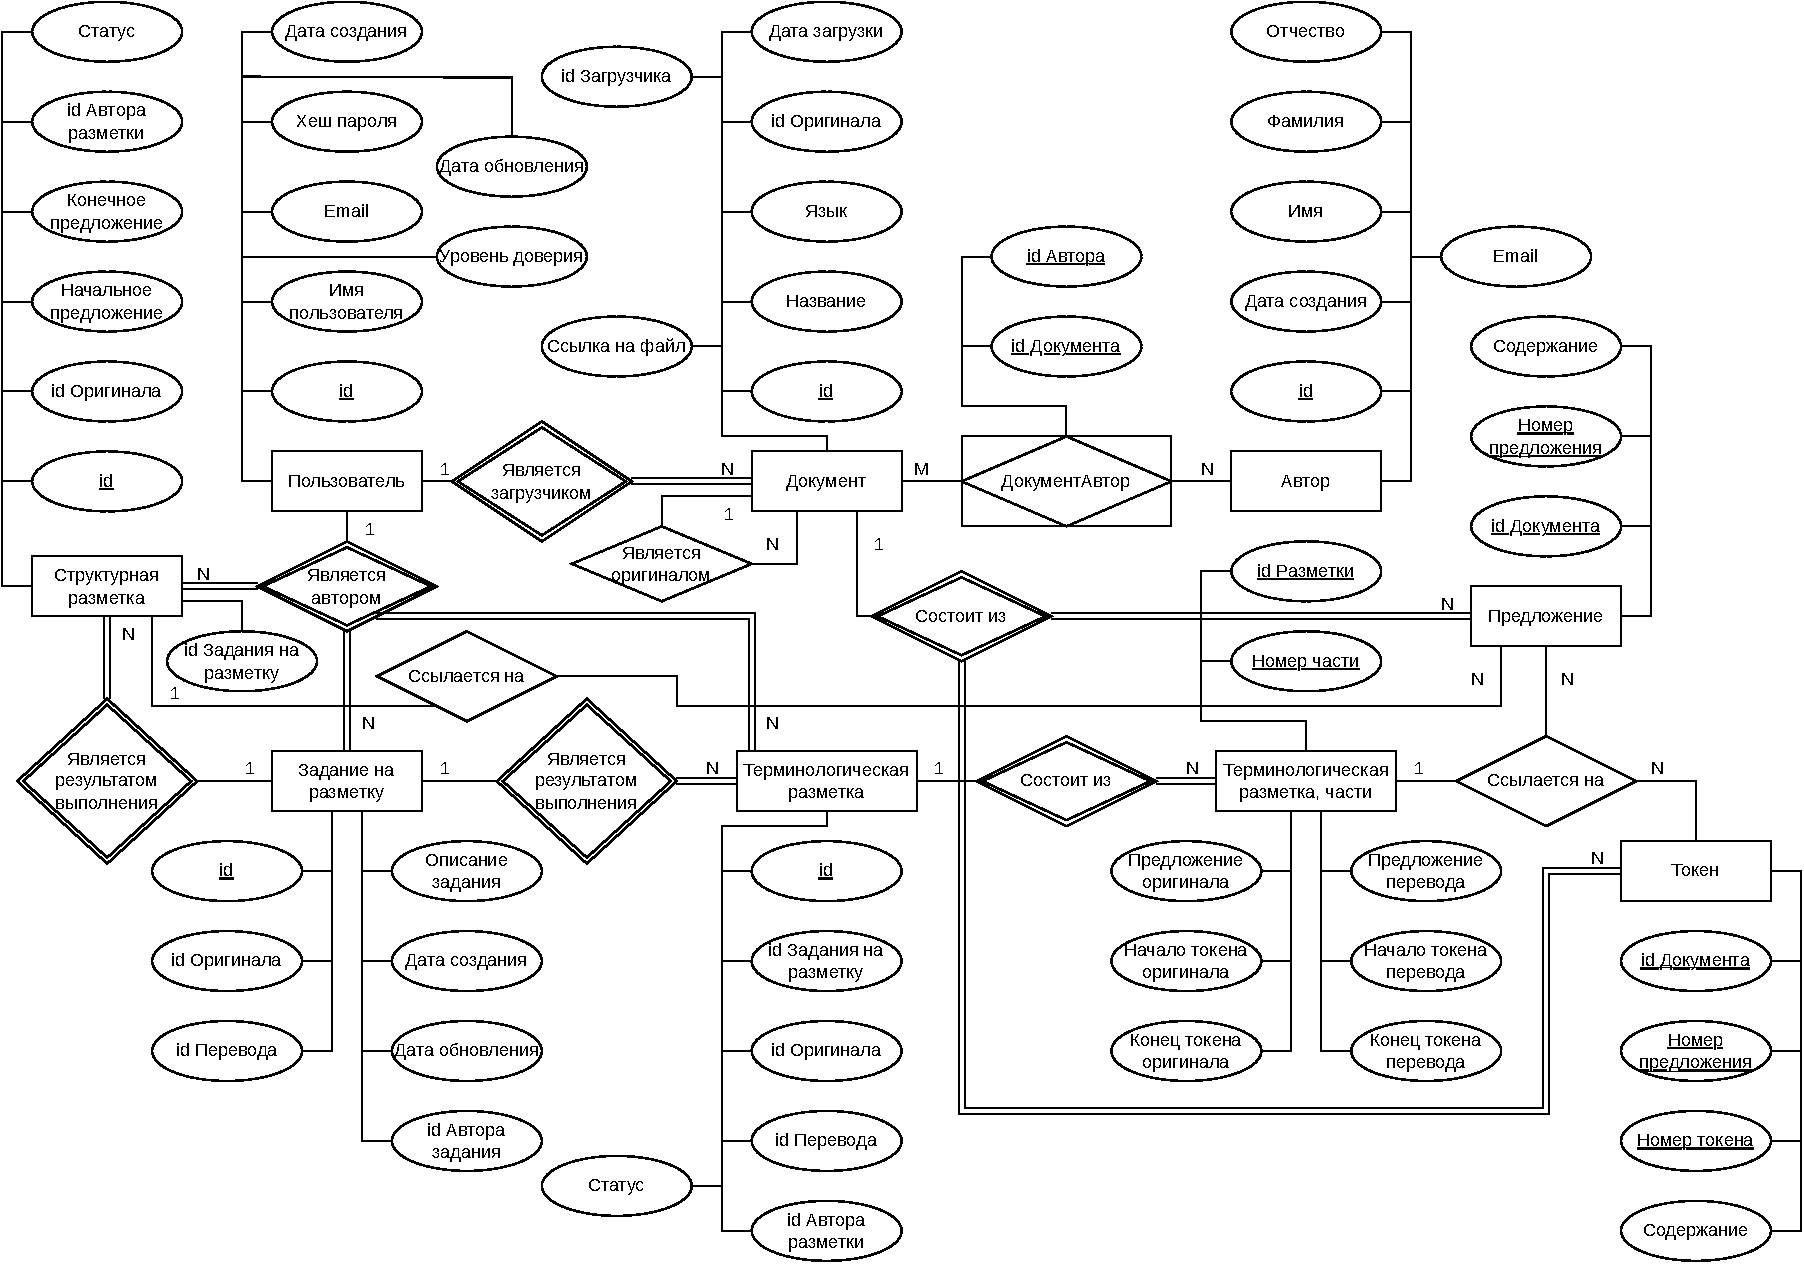
\includegraphics[angle=90, width=\textwidth]{diag/chen.pdf}
	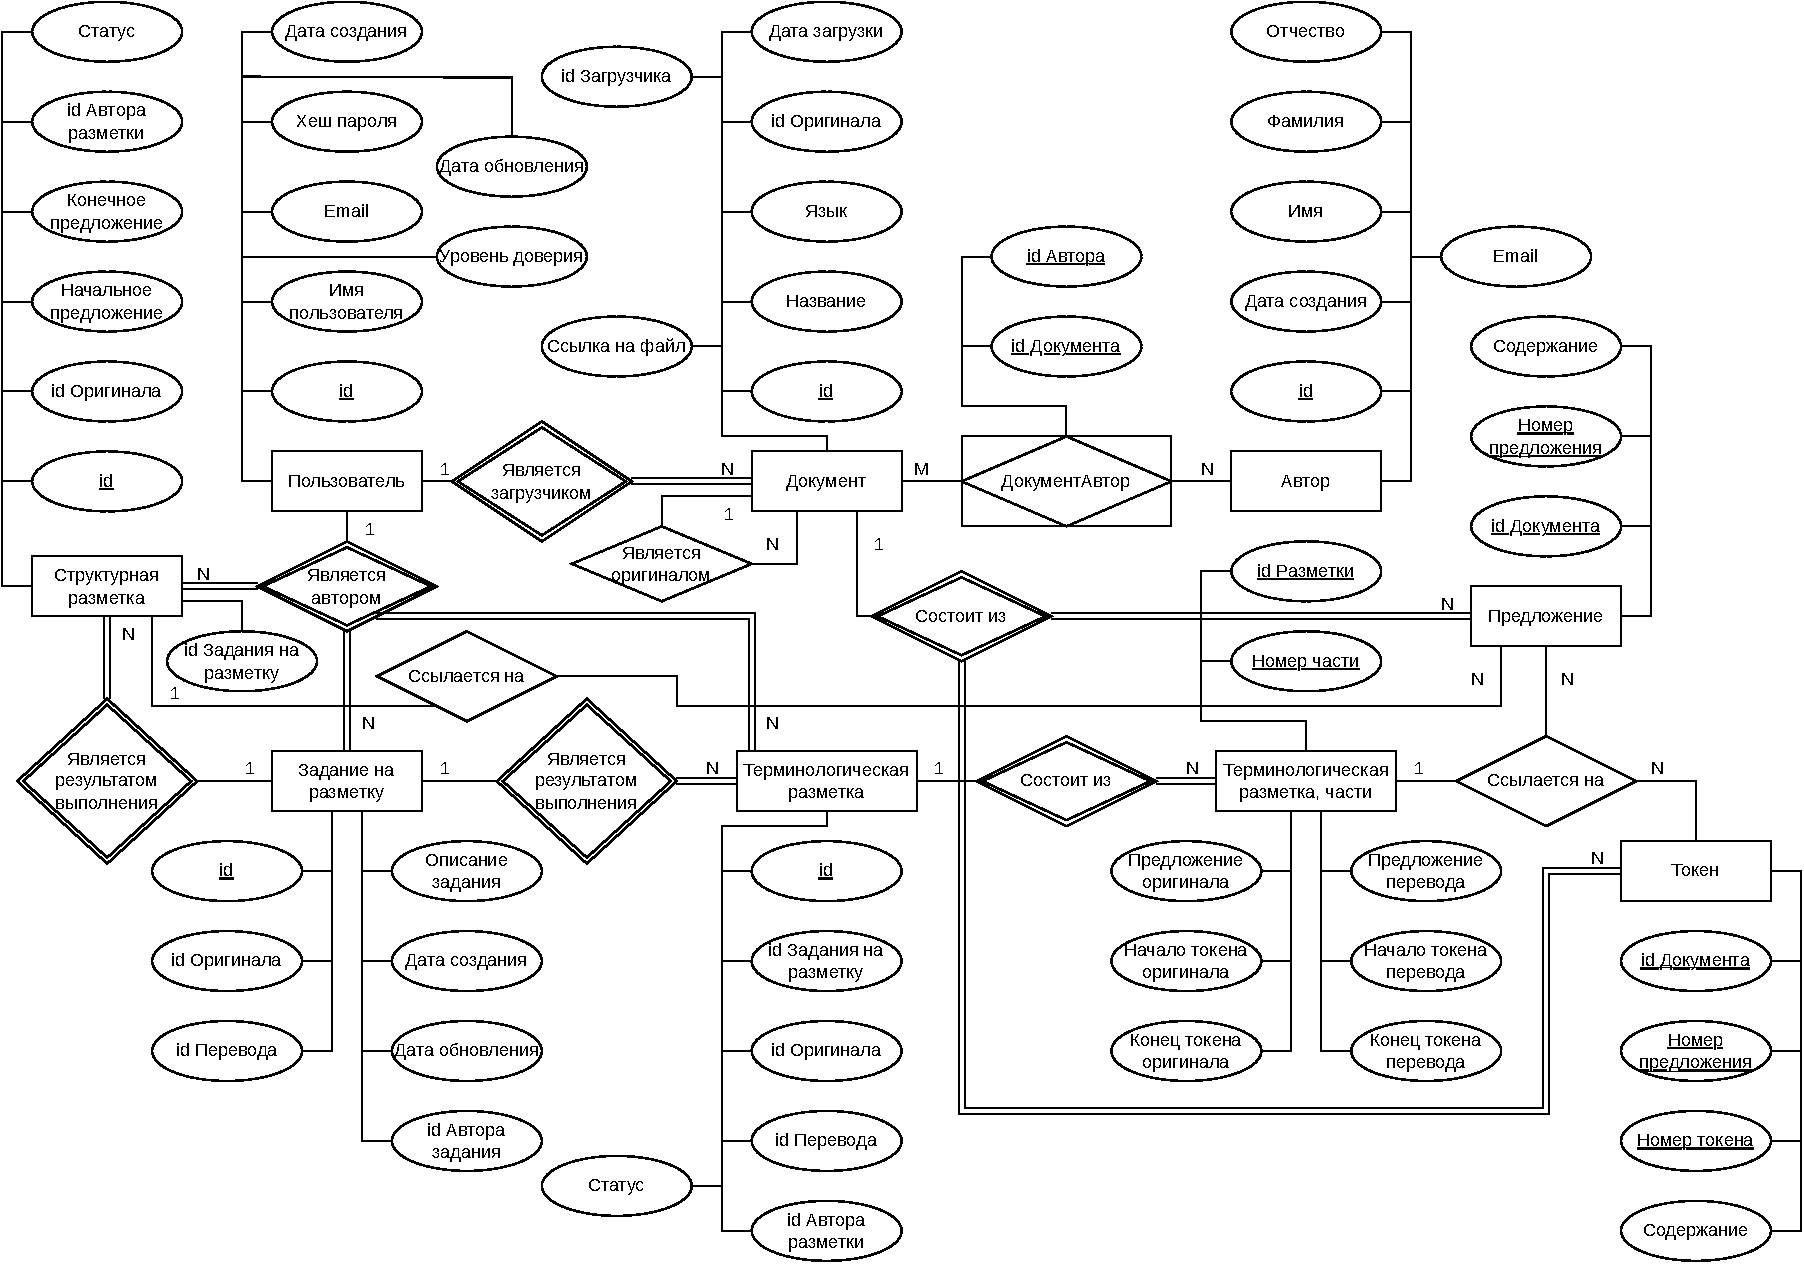
\includegraphics[width=\textwidth]{diag/chen.pdf}
	\caption{ER-диаграмма в нотации Чена}
	\label{fig:chen}
\end{figure}

Сценарий использования системы может быть следующий:
\begin{enumerate}
    \item Администратор загружает документ в систему, перед этим заполнив метаинформацию о нем --- язык, название текста, информацию об авторах.
    \item Из документа извлекаются предложения и добавляются в таблицу <<Предложение>> базы данных со ссылкой на документ, которому они принадлежат.
    \item Производится токенизация загруженного текста, токены добавляются в таблицу <<Токен>> базы данных, со ссылкой на документ и предложение, которым токен принадлежит.
    \item Модератор создает задание на разметку, указав документы (оригинал и перевод), которые требуется разметить, а также добавив словестное описание задания.
    \item Пользователь видит новое задание и приступает к разметке --- сопоставляет части текста одного документа с соответствующими им частями текста другого документа.
    \item По завершении разметки, пользователь отправляет ее на проверку модераторам.
    \item Модераторы проверяют разметку пользователя и либо утверждают, либо отклоняют ее. В случае утверждения разметки, у пользователя увеличивается рейтинг доверия.
\end{enumerate}

% \textbf{Диаграмма сущностей базы данных}

\textbf{Заключение}

В данной статье были рассмотрены актуальные проблемы, с которыми сталкиваются участники разметки параллельных корпусов технических текстов, описана функциональность информационной системы, позволяющей организовать удобную работу множества участников разметки, выделены сущности базы данных для описанной информационной системы и приведен сценарий ее использования.
% А также была достигнута цель данной статьи --- создание диаграммы сущностей базы данных для описанной информационной системы.

% Список литературы
\noindent
\textbf{Список литературы}
% \nocite{*}
\bibliographystyle{modified-utf8gost705u}
\begingroup
\renewcommand{\section}[2]{}
% \raggedright
\bibliography{bibliography}
\endgroup

% \renewcommand\refname{}
% \begingroup
% \bibliographystyle{modified-utf8gost705u}
% \raggedright
% \bibliography{bibliography}
% \endgroup

% \newpage

\end{document}
